
\bigskip

\subsection{Tuning anisotropic networks to specific distance-dependent
  connection probabilities}
\label{sec:tuned_networks}


In tuned anisotropic graphs, the form of the width function $w(x)$
determines the distance-dependent connection probability $C(x)$ in the
network. Here, we are interested in determining $w(x)$ such that
$C(x)$ matches the probabilities as found by \textcite{Perin2011}.

In general, let $C(x): [0,\sqrt{2}) \to [0,1]$ be a distance-dependent
  connection probability on the unit square. From

  \begin{figure}[h!]
    \centering
    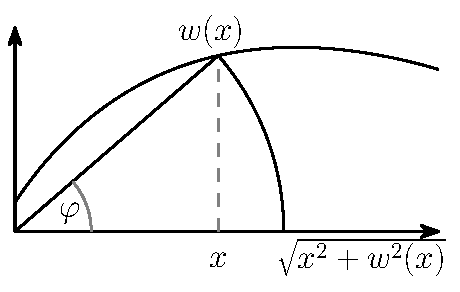
\includegraphics[width=0.35\textwidth]{%
    img/distance-dependent-relation-in-tuned-networks.pdf} %
  \end{figure}

 we obtain the relation
%
\begin{align}
C\left(\sqrt{x^2+w^2(x)}\right) = \frac{1}{\pi} \operatorname{arctan}
\frac{w(x)}{x}. \label{eq:geo_rel}
\end{align}
%
In order to solve for $w(x)$ we approximate $\sqrt{x^2 + w^2(x)}
\approx x$, which inserting into \eqref{eq:geo_rel} yields
\begin{equation}
C(x) \approx \frac{1}{\pi} \operatorname{arctan} \label{eq:tanapprox}
\frac{w(x)}{x}.
\end{equation}
%
Under the assumption that $C(x)<\frac{1}{2}$ for all $x \in
[0,\sqrt{2})$ we obtain the identity
\begin{equation}
  w(x) = x \tan\left( \pi\, C(x) \right). \label{eq:xtan}
\end{equation} 
%
With the distance-dependent connection probabilities
\begin{align}
  C(x) = -0.00142\, \left(0.00276 + x^{-0.945}\right)^{-1} + 0.23079
  \label{eq:perin_c}
\end{align}
%
extracted from \textcite{Perin2011} we can now use \eqref{eq:xtan} to
obtain $w(x)$. However, Perin et al.~mapped connectivity in layer 5 of
the rat's somatosensory cortex up to a distance of
$\SI{300}{\micro\meter}$ and $x$ was measured in \SI{}{\micro\meter}
in \eqref{eq:perin_c}. Thus, to obtain a reasonable connection
density, we finally need adjust the side length of the square
surface. We found that with a side length $E=\SI{296}{\micro\meter}$ a
connection of density of $p=0.116$ is achieved. With this, the width
$w(x)$ obtained from inserting \eqref{eq:perin_c} into \eqref{eq:xtan}
generates tuned anisotropic networks with a distance-dependent
connection probability matching the results from \cite{Perin2011}
(Fig.~\ref{MAIN-fig:4_net_models}H).


%% %% \begin{figure}[htp]
%% %%   \centering
%% %%   \makebox{%
%% %%     \begin{overpic}[height=4.05cm]{%
%% %%         plots/6154302f.pdf}
%% %%       \put(85.5,57.0){\small\textbf{A}}
%% %%       %\put(12,5){\small\textbf{A}}
%% %%     \end{overpic}
%% %%     \hfill
%% %%     \begin{overpic}[height=3.955cm]{%
%% %%         plots/ef0e785d.pdf}
%% %%       \put(88.5,58.2){\small\textbf{B}}
%% %%     \end{overpic}
%% %%   }%
%% %%   \captionsetup{skip=7pt}
%% %%   \caption{\textbf{Network side length adjusted to match overall
%% %%       connection probability} Side length of the network's surface
%% %%     determines the overall connection probability in the network when
%% %%     axon width function $w(x)$ is fixed. \textbf{A)} Connection
%% %%     probability declines with rising side length \textbf{B)}
%% %%     Determining side length as $s=\SI{296}{\micro\meter}$ to match $p
%% %%     = 0.116$ as reported by \textcite{Song2005}. (\smtcite{6154302f},
%% %%     \smtcite{ef0e785d})}
%% %%   \label{fig:determine_side_length}
%% %% \end{figure}



%% Having determined the neotwork's side length $s$, we're extending the
%% quiver of generated sample networks for the numerical analysis once
%% more by the \enquote{tuned anisotropic graphs}\index{tuned
%%   anisotropic networks}, in which the axon width $w(x)$ was determined
%% such that the networks reflect Perin's connectivity profile. Analyzing
%% the obtained axon width function we note that $x \gg w(x)$ holds for
%% most $x$, justifying the approximation
%% \[
%%   \sqrt{x^2 + w^2(x)} \approx x
%% \] 
%% \textit{a posteriori} (\autoref{fig:perin_axwidth}). From the 25
%% generated networks overall connection probability is extracted as $p =
%% 0.1160 \pm 0.0006$ (SEM), as expected from the choice of $s$
%% (\smtcite{f11dca65}).



%% % This approximation holds well as long as $x \gg w(x)$. Using the
%% % relation to tune the axon width to produce anisotropic networks with a
%% % distance-dependency as reported by Perin et al., we find that for all $x$ is
%% % strictly greater than $w(x)$  %(\autoref{fig:perin_axwidh


%% \begin{figure}[htp]
%%   \centering
%%   \hspace{0.05cm}
%%   \begin{overpic}[width=0.6\textwidth]{%
%%       plots/d45c02e4.pdf}
%%           \put(69.4,51.5){\small\textbf{A}}
%%   \end{overpic}
%%   \hfill
%%   \begin{overpic}[width=0.35\textwidth]{%
%%       plots/8f0d65e4.pdf}
%%     \put(81,86){%
%%       \fboxsep=2pt\colorbox{white}{\small\textbf{B}}
%%     }
%%   \end{overpic}
%%   \captionsetup{skip=7pt}
%%   \caption{\textbf{Anisotropic network model with tuned axon width
%%       $\mathbf{w(x)}$} \textbf{A)} Resulting axon width function
%%     $w(x)$ from tuning to distance-dependent connection profile as
%%     reported by \textcite{Perin2011}, see also
%%     \autoref{fig:perin_profiles}. Note that $x \gg w(x)$ for most $x$,
%%     supporting approximation~\ref{eq:tanapprox}. \textbf{B)}
%%     Showing for a single neuron (star) connected (red) and unconnected
%%     (gray) neurons in the tuned anisotropic network, revealing
%%     the characteristic axon shape. (\smtcite{d45c02e4}, \smtcite{8f0d65e4})}
%%   \label{fig:perin_axwidth}
%% \end{figure}




%% Overall distance-dependent connection probabilities in the tuned
%% an\-iso\-tro\-pic graphs clearly match the profile of Perin et
%% al.~(\autoref{fig:perin_profiles} A), presenting strongest the
%% argument in support of the chosen approximation. Analyzing two neuron
%% connections \marginpar{revisiting two neuron connections} in the tuned
%% networks, we affirm the findings of the last section. In their
%% experiment, Perin et al.~were able to show an overrepresentation of
%% reciprocal connections at any inter-neuron distance
%% (\autoref{fig:perin_profiles} B-C). Rather than matching these
%% profiles, we find that occurrences of one- and bidirectionally
%% connected pairs in the anisotropic graphs align with probabilities
%% obtained from the distance-dependent overall connection probability
%% $p(x)$ under the assumption of independence (cf. Equation~\ref{eq:pairs}),
%% \begin{equation*}
%%   \label{eq:pairs}
%%   \begin{aligned}%
%%     & \mathbf{P}_{X=1}(x) = 2p(x) \left(1-p(x) \right)    
%%       && \text{single connection,}\\
%%     & \mathbf{P}_{X=2}(x) = p(x)^2        
%%       &&\text{reciprocal connection.}
%%   \end{aligned}%
%% \end{equation*}%
%% \vspace{0.1cm}%
%% Thus, in comparison with Perin et al.'s findings, we find that
%% anisotropy in connectivity cannot account for the overrepresentation
%% in reciprocal connections. While results in
%% Section~\ref{sec:two_neuron} still indicated such an
%% overrepresentation due to distance-dependency, examining the
%% occurrence of two neuron connections at any inter-neuron distance in
%% anisotropic networks, tuned to a distance-dependent connection profile
%% matching experimental findings from cortical circuits, imply complete
%% unrelatedness of anisotropy and two-neuron connection distributions.

%% \begin{figure}[htp]
%%   \centering
%%   \makebox{%
%%     \begin{overpic}[width=0.5\textwidth]{%
%%         plots/875505b0_overall.pdf}
%%       \put(28,19){\small\textbf{A}}
%%     \end{overpic}
%%     \hfill
%%     \begin{overpic}[width=0.5\textwidth]{%
%%         plots/875505b0_single.pdf}
%%       \put(28,19){\small\textbf{B}}
%%     \end{overpic}
%%   }%
%%   \vspace{-0.6cm}
%%   \makebox{%
%%     \begin{overpic}[width=0.5\textwidth]{%
%%         plots/875505b0_recip.pdf}
%%        \put(28,19){\small\textbf{C}}
%%     \end{overpic}
%%     \vspace{-1cm}
%%     \includegraphics[width=0.5\textwidth]{%
%%       img/tuned_legend.pdf}   
%%   }%
%%   \captionsetup{skip=7pt}
%%   \caption{\textbf{Distance-independent overrepresentation of
%%       reciprocal connections} Comparison of occurrences of one- and
%%     bidirectionally connected neuron pairs in the tuned anisotropic
%%     networks (gray) with profiles found by Perin et al.~(red), shows
%%     that overrepresentation of bidirectional pairs is
%%     distance-independent and not connected to anisotropy.  \textbf{A)}
%%     Overall connection probability in the tuned anisotropic networks
%%     was successfully adjusted to reflect connection probability found
%%     by Perin et al. \textbf{B)-C)} Showing in blue the probabilities
%%     to obtain a neuron pair motif (single edge in B, two edges in C)
%%     calculated under independence assumption from the overall
%%     probability from A), we find that counts in the tuned anisotropic
%%     networks (gray) match the independence assumption and do
%%     \textit{not} show the overrepresentation present in Perin et al.'s
%%     experiment. (\smtcite{875505b0})}
%%   \label{fig:perin_profiles}
%% \end{figure}





 %%%%% ------------------------------


   
  
%% For this we introduce anisotropic networks tuned to reflect a given
%% distance-dependent connection profile $C(x)$. We are facing the
%% following problem: Given $C(x):[0,\sqrt{2}) \to [0,1]$, find
%% $w:[0,\sqrt{2}) \to [0,\infty)$ such that the probability to have a
%% connection from $v_1$ to $v_2$ for arbitrary vertices $v_1 \neq v_2$
%% in an anisotropic graph $G(n,w)$ with distance $\mathrm{d}(v_1,v_2) =
%% x$ is $C(x)$. The problem is in general highly complex when nothing
%% can be assumed about $C(x)$. We find an approximate solution to the
%% problem considering the following geometric relation:

%% \begin{figure}[htp]
%%   \centering
%%   \makebox{%
%%     \begin{overpic}[height=3.35cm]{%
%%         plots/bed7650b.pdf}
%%     \end{overpic}
%%   }%
%%   \caption{Computing connection probability $C(x)$ from non-constant
%%     $w(x)$}
%%   \label{fig:dpp_wc}
%% \end{figure}
